\section{Design}
\subsection{Overall System Architecture}
\begin{figure}[h!]
\centering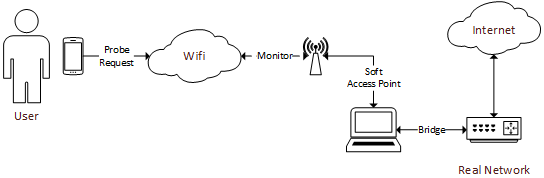
\includegraphics{design/figures/overall.png}
\caption{Overall system architecture.}
\end{figure}
A soft access point is created on the detection of a valid, open encryption, probe request, and the network traffic is bridged to an actual network to ensure that the user is still able to access the internet, and the attacker can monitor passing traffic.

\subsection{Class Diagrams}
\subsubsection{Android Game}
The Android game design is relatively simple. It consists of two classes that inherit from the libgdx screen class, with the GameScreen class holding the GameRenderer and GameWorld which renders and holds the game state respectively doing the majority of the work.
\clearpage
\begin{figure}[h!]
\centering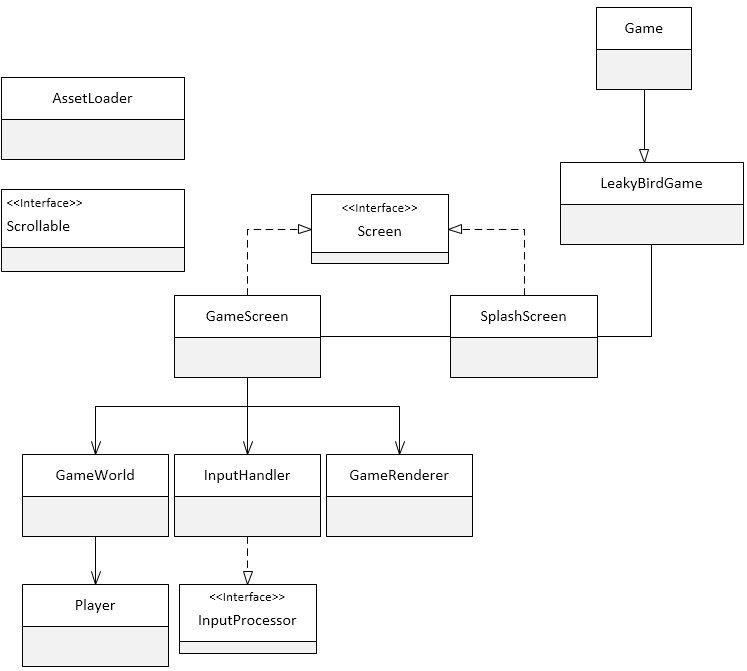
\includegraphics{design/figures/ag-cd.png}
\caption{Android game class diagram.}
\end{figure}

\subsection{Android Location Provider}
To successfully use platform specific functionality within the libgdx game environment an interface needs to be created to allow use of the functions. More detail on this can be found in the implementation section; however, below details the classes required to provide the game with the ability to get location information from the Android device.

\begin{figure}[h!]
\centering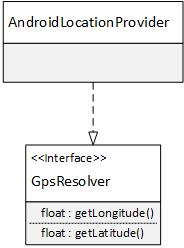
\includegraphics{design/figures/ag-lp-cd.png}
\caption{Android game libgdx location interface.}
\end{figure}

\clearpage